\documentclass{article}

\usepackage{authblk}
\usepackage{blindtext}
\usepackage{graphicx}
\usepackage[capposition=top]{floatrow}
\usepackage{float}

\usepackage[
    backend=biber,
    style=apa,
    url=false,
    doi=false,
    sorting=ynt,
    eprint=false 
]{biblatex}
\addbibresource{two_references.bib}

\title{Pseudo Article}
\date{November 2021}

\author[1]{Yue Min \thanks{This is the actual author}}
\affil[1]{Uiversity of Zurich}

\author[2]{Second Author \thanks{This is a pseudo author}}
\affil[2]{Second Affliation}

\begin{document}
\maketitle

\section*{Abstract}
This is an abstract section. \blindtext

\newpage

\section{Figure Paragraph}
This is a paragraph with Figure \ref{fig:sens}. \blindtext[2]\\

\begin{figure}[H]
    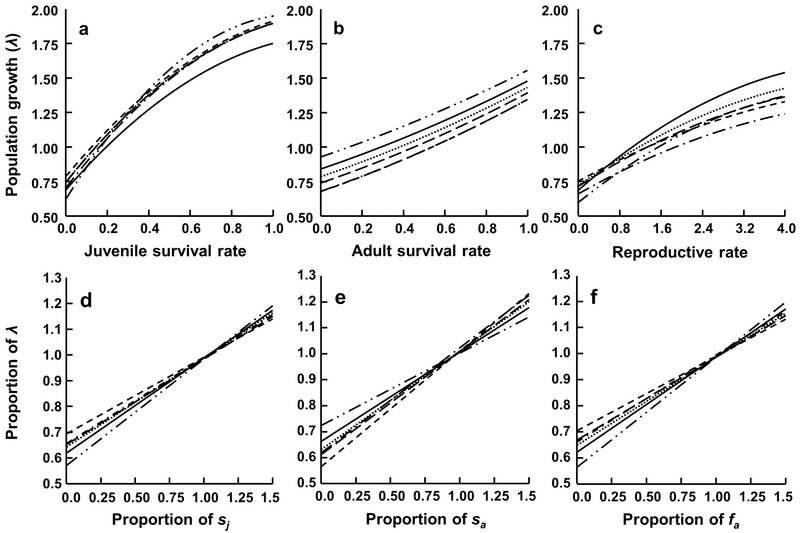
\includegraphics[width=0.7\textwidth]{sensitivity.png}
    \centering
    \caption{Sensitivity of Population Growth}
    \floatfoot{Note: From Ryberg, Wade \& Hill, Michael \& Painter, Charles \& Fitzgerald, Lee. (2015). Linking irreplaceable landforms in a self-organizing landscape to sensitivity of population vital rates for an ecological specialist: Landform-Dependent Species Demography. Conservation biology : the journal of the Society for Conservation Biology. 29. 10.1111/cobi.12429. Figure 2.}
    \label{fig:sens}
\end{figure}

\section{Table Paragraph}
This is a paragraph with Table \ref{tab:birth}. \blindtext[1]

\begin{table}[h]
    \begin{tabular}{|l|c|c|c|}
    \hline
    Year & \begin{tabular}[c]{@{}c@{}}Birth rate \\ (per 1000)\end{tabular} & \begin{tabular}[c]{@{}c@{}}Population rate \\ (per 1000)\end{tabular} & Total fertility rate \\ \hline
    1990 & 12.1                                                             & -0.40                                                                 & 1.81                 \\ \hline
    1995 & 8.6                                                              & -5.00                                                                 & 1.23                 \\ \hline
    2000 & 9.0                                                              & -5.10                                                                 & 1.27                 \\ \hline
    2001 & 8.6                                                              & -5.60                                                                 & 1.24                 \\ \hline
    2002 & 8.5                                                              & -5.80                                                                 & 1.21                 \\ \hline
    2003 & 8.6                                                              & -5.70                                                                 & 1.23                 \\ \hline
    2004 & 9.0                                                              & -5.20                                                                 & 1.29                 \\ \hline
    2005 & 9.2                                                              & -5.40                                                                 & 1.31                 \\ \hline
    2006 & 9.6                                                              & -5.10                                                                 & 1.38                 \\ \hline
    2007 & 9.8                                                              & -5.00                                                                 & 1.42                 \\ \hline
    2008 & 10.2                                                             & -4.3                                                                  & 1.48                 \\ \hline
    \end{tabular}
    \caption{Birth Rate, Population Growth Rate and Total Fertility Rate}
    \floatfoot{Note: From Petkov, Georgi \& Marinova, J \& Chakarova, P \& Dimitrova, Sv \& Yordanov, G \& Peeva, Katya \& Parashkevova, Boryana \& Chamova, Galya \& Marinov, V \& Zdravkova, J. (2010). DYNAMICS OF SOME BASIC DEMOGRAPHIC INDICATORS IN BULGARIA FOR THE LAST CENTURY. Trakia Journal of Sciences. 8. 453-465. Table 2.}
    \label{tab:birth}
\end{table} 



\noindent This is the first citation: \cite{Kozlowski2020}. This is the second citation: \cite{gormsen2020}.

\newpage
\printbibliography


\end{document}